%
% dual.tex -- duale unterteilung
%
% (c) 2019 Prof Dr Andreas Müller, Hochschule Rapperswil
%
\section{Dualzahlen-Unterteilung%
\label{section:dualzahlen}}
\rhead{Dualzahlen}
Wir beginnen mit der Unterteilung
\[
U_0
=
\{ k\,|\, k\in\mathbb Z\}
=
\mathbb Z
\]
der reellen Achse durch ganze Zahlen.
Man könnte auch sagen, als Masseinheit auf der $x$-Achse wird die
Länge des Abtastintervals verwendet.
Abtastung erfolgt also nur an ganzzahligen $x$-Werten und
Translationen um ganze Zahlen sind uneingeschränkt möglich.

\begin{figure}
\centering
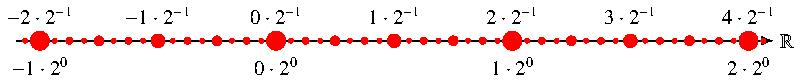
\includegraphics{chapters/3-haar/images/dual.pdf}
\caption{Dualzahlen-Unterteilung $\mathbb D$ von $\mathbb R$ durch
rationalen Zahlen mit Nennern, die Zweierpotenzen sind. 
Abtastung auf den Dualzahlen ermöglicht beliebige Translationen um
Vielfache einer Zweierpotenz und Skalierungen um Zweierpotenzen.
\label{haar:figure:dualzahlen}}
\end{figure}
Um mehr Detail zu erhalten, kann das Abtastinterval halbiert werden.
Die Unterteilung bekommt dann die Form
\[
U_1
=
\{ k2^{-1}\,|\, k\in\mathbb Z\}
=
2^{-1}\mathbb Z.
\]
Offenbar können damit doppelt so hohe Frequenzen abgetastet werden.
Beim Übergang von $U_0$ zu $U_1$ können die bereits bekannten Samples
an den Stellen $U_0$ weiterverwendet werden.
In $U_1$ sind Translationen um ganzzahlige Vielfache von $\frac12$ 
möglich.

Der Verfeinerungsprozess kann weitergeführt werden, so dass beliebig
feine Unterteilung
\[
U_j = \{ k2^{-j}\,|\,k\in\mathbb Z\}
\]
entstehen (Siehe auch Abbildung~\ref{haar:figure:dualzahlen}).
In jedem Schritt wird die Menge an Informationen der gesampelten Funktion
verdoppelt, ohne dass früher gefundene Samples nutzlos werden.
In $U_j$ sind Verschiebungen um ganzzahlige Vielfache von $2^{-j}$ 
möglich.
Es wird daher in $U_j$ nicht nur möglich, Signale für genügend grosses $j$
beliebig genau zu approximieren, sondern auch beliebig fein aufgelöste
Translationen abzubilden.
Wir bezeichnen den Vektorraum der stückweise konstanten Funktionen
bezüglich der Unterteilung $U_j$ mit $V_j$.
Es gilt also $V_j \subset V_{j+1}$.

Die Mengen $U_j$ haben zusätzliche Struktur.
Die Addition und die Multiplikation mit ganzen Zahlen führt nicht aus
der Menge heraus.
Sind $x=k_x2^{-j}\in U_j$ und $y=k_y2^{-j}\in U_j$ und $r\in\mathbb Z$,
dann gilt
\begin{align*}
x+y &= k_x 2^{-j}+k_y2^{-j}=(k_x+k_y)2^{-j}\in U_j
\\
rx&=r(k_x2^{-j}) = (rk_x)2^{-j}\in U_j.
\end{align*}
Man sagt, $U_j$ ist ein {\em Modul} über den ganzen Zahlen oder ein
{\em $\mathbb Z$-Modul}.
Die Additionseigenschaft ist insofern von Bedeutung, als eine analoge
Eigenschaft für die Konstruktion der Fouriertheorie von entscheidender
Bedeutung war.

Man kann auch versuchen, eine Basis zu konstruieren.
Im Vektorraum $V_j$ können die Funktionen mit Samplewerten
\[
e^{(l)}_k = \frac{1}{2^{-j/2}}\delta_{kl}
\]
als Basisvektoren verwendet werden.
Wegen
\[
\langle e^{(l)},e^{(r)}\rangle
=
2^{-j}
\biggl(
\frac{1}{2^{-j/2}}
\biggr)^2\delta_{lr}
=
\delta_{lr},
\]
Jeder einzelne der Vektorräume $V_j$ hat also eine einfach anzugebende
Basis.

Die Vereinigung aller $U_j$ 
\[
\mathbb D
=
\bigcup_{j=0}^\infty U_j
=
\{ ke^{-j}\,|\, k\in\mathbb Z, j\in\mathbb N\}
\subset
\mathbb Q
\]
ist die Menge aller Brüche mit Zweierpotenz-Nennern.
Sie heisst die Menge der {\em Dualzahlen}.


Ausser der Addition hat 
$\mathbb D$ noch weitere Struktur.
Sind $x = k_x2^{-j_x}\in U_{j_x}$ und $y=k_y2^{-j_y}\in U_{j_y}$, dann
ist das Produkt
\[
xy = k_x2^{-j_x} k_y2^{-j_y}=(k_xk_y)2^{-(j_x+j_y)}\in U_{j_x+j_y}
\]
und damit $xy\in\mathbb D$.
In den Dualzahlen ist daher auch die Multiplikation möglich, so wie
dies in der Mengen $\mathbb Z$ der ganzen Zahlen möglich ist.
Man sagt, $\mathbb D$ ist ein Ring.
Während in jeder Menge $U_j$ nur die Multiplikation mit ganzen Zahlen
möglich war, ist in $\mathbb D$ auch die Division durch Zweierpotenzen
möglich.
Damit ist in $\mathbb D$ die Möglichkeit entstanden, die Abtastung
in Zweierpotenzschritten beliebig zu verfeinern.

Die stückweise konstanten Funktionen mit Teilpunkten in der Menge
$\mathbb D$ bilden einen Vektorraum, den man aus der Vereinigung
der Vektorräume $V_j$ aufbauen kann.
Wir bezeichnen mit
\[
V_\infty = \bigcup_{j=1}^\infty V_j 
\]
den Unterraum des Vektorraumes der stückweise konstanten Funktione mit
dem Skalarprodukt.
Mit diesen speziellen stückweise konstanten Funktionen lassen sich ebenfalls
beliebige stetige Funktionen approximieren, denn dazu war ja nur 
erforderlich, dass sich das Korn der Unterteilung, also $2^{-j}$ im Falle
von $V_j$ beliebig klein machen lässt.

Die Konstruktion ist aber trotzdem nicht befriedigend.
Zum einen sind die Funktionen $e^{(k)}$ der verschiedenen Vektorräume
nicht orthogonal.
Andererseits lösen sie das bereits angesprochen Problem der Redundanz
der Information nicht.
Das Skalarprodukt eines Signals mit der stückweise konstanten Funktion
$e^{(l)}$ ist im Wesentlichen der Abstastwert in der Nähe von $l2^{-j}$.
Für langsam veränderliche Signale sind nahe beeinander liegende 
Abtastwerte nahe beeinander.
Mit den Vektorräumen $V_j$ ist es also möglich, ein Signal beliebig
genau abzutasten, aber die naheliegende Basis führt nicht zu einer
effizienten Charakterisierung des Signals.

%Die Funktionen $\psi_{l,j}$ erfassen also genau die Details, die beim
%Abtasten mit der feineren Unterteilung mit Korn $2^{-j-1}$ erkennbar
%werden.
%Aber warum bei $U_0$ beginnen?
%Der Mittelwert zweier benachbarter Abtastwerte sagt bereits einiges
%über die Werte aus, der Unterschied dieser Werte ist aber das, was
%was erst in der Abtastung mit ganzzahligen Abtastpunkten erkennbar wird.
%Wir könnten also auch mit $U_{-1}$ beginnen, der Unterteilung
%\[
%U_{-1} = \{\dots -4,-2,0,2,4,6,8,\cdots\},
%\]
%und der Menge $V_{-1}$ der stückweise konstanten Funktionen mit
%Sprungestellen bei geraden Zahlen.
%Doch warum da aufhören: Es gibt eine Zerlegung des Raums der stückweise
%konstanten Funktionen mit Sprungstellen in $\mathbb D$ in Form einer
%Kette
%\begin{equation}
%\{0\}
%\subset
%\dots
%\subset
%V_{-2}\subset V_{-1} \subset V_{0} \subset V_{2} \subset\dots\subset
%V_j \subset V_{j+1}\subset\dots \subset V_{\infty}
%\label{haar:kette}
%\end{equation}
%mit folgenden zum Teil noch nachzuweisenden Eigenschaften:
%\begin{enumerate}
%% XXX Problem approximation
%\item
%Jede stückweise konstante Funktion lässt sich beliebig genau
%durch Funktionen aus $V_j$ approximieren, also
%\[
%\bigcup_{j\in\mathbb Z} V_j = V_\infty
%\]
%\item
%Es gibt eine orthonormierte Familie von Funktionen $\psi_{l,j}\in V_{j+1}$
%die auf $V_j$ orthogonal sind, und die genau das erfassen, was in $V_{j+1}$
%gegenüber $V_j$ dargestellt werden kann.
%Etwas formaler: die $\psi_{l,j}$ spannen einen Unterraum
%$W_{j} = \langle \psi_{l,j}\,|\, l\in\mathbb Z\rangle \subset V_{j+1}$
%auf derart, dass
%\[
%V_{j+1} = V_j \oplus W_j.
%\]
%\item 
%Die Funktionen $\psi_{l,j}$ sind Translate einer einzigen Funktion.
%Die Funktion $\psi_{l,j}$ ist die Verschiebung der Funktion $\psi_{0,j}$ 
%um $l2^{-j}$.
%\item
%Die Funktionen $\psi_{0,j}$ sind Streckung der Funktion
%$\psi_{0,0}$ um den Faktor $2^{-j}$, die wir auch mit
%$\psi(x)=\psi_{0,0}(x)$ bezeichnen wollen:
%\[
%\psi_{0,j}(x) = \frac1{2^{j/2}}\psi_{0,0}(2^jx).
%\]
%$\psi$ heisst das {\em Mutter-Wavelet}.
%\item 
%Nur für die Nullfunktion verschwinden alle Abtastungen mit Funktionen
%$\psi_{l,j}$, oder etwas formeller:
%\[
%\bigcap_{j\in\mathbb Z} = \{0\}.
%\]
%\end{enumerate}
%
%Die Konstruktion der Funktionen $\psi$ zeigt aber noch eine weitere 
%Besonderheit, die später von Nutzen sein wird.
%Die $\psi$-Funktionen wurden als Differenzen von charakteristischen
%Funktionen von Intervallen aufeinanderfolgenden Endpunkten in $U_{j+1}$
%aufgebaut.
%Alle diese charakteristischen Funktionen sind verschobene und geeignet
%gestreckte Versionen der charakteristischen Funktion des Grundintervals
%$[0,1)$.
%Setzen wir
%\[
%\varphi(x) = \chi_{[0,1)} (x),
%\]
%dann ist
%\[
%\chi_{[l2^{-j},(l+1)2^{-j})}(x)
%=
%\varphi((x-l2^{-j})2^j).
%\]
%% XXX Begründung
%Und auch die Funktion $\psi_{0,0}$, aus der sich alle $\psi_{l,j}$ durch
%Streckung und Verschiebung gewinnen lassen, lässt sich aus $\varphi$
%aufbauen:
%\begin{equation}
%\psi_{0,0}(x) = \varphi(2x) - \varphi(2x - 1).
%\label{haar:psiphi}
%\end{equation}
%Die Funktion $\varphi$ heisst auch das {\em Vater-Wavelet}.
%Das Vater-Wavelet $\varphi$ erfüllt eine ähnliche Relation
%wie \eqref{haar:psiphi}.
%Bei der Konstruktion haben wir diese Relation sogar in entscheidender
%Weise gebraucht, indem wir das Interval in zwei Halbintervalle aufgeteilt
%haben.
%Diese Aufteilung bedeutet
%\[
%\varphi(x) = \varphi(2x) + \varphi(2x-1),
%\]
%bis auf das Vorzeichen des zweiten Summanden dasselbe wie 
%\eqref{haar:psiphi}.
%
%Aus diesem Beispiel können wir einen Plan für die Konstruktion allgemeinerer
%Wavelet-Basen ableiten.
%Wir hätten gerne eine Aufteilung des interessiernden Funktionenraumes
%in Form einer Kette \eqref{haar:kette} derart, dass die ``Zwischenräume''
%$W_j$ eine Orthonormalbasis haben, die aus verschobenen und gestreckten
%Kopien
%$\psi()$
%einer einzigen Funktion $\psi$, dem Mutter-Wavelet, besteht.
%Das Mutter-Wavelet ist eine Linearkombination von verschobenen
%und skalierten Kopien des Vaterwavelets $\varphi(x)$, welches seinerseits
%eine Linearkombination von verschobenen und skalierten Kopien seiner
%selbst ist.
%Die Koeffizienten der Linearkombinationen für $\psi$ und $\varphi$ sind
%bis auf die Vorzeichen identisch.
%
%
%
%
